\documentclass[10pt,a4paper]{report}

\usepackage{style}

\title{\Huge{\textbf{Le Taquin}}}
\author{Mélanie MARQUES \& Guillaume COQUARD}
\date{Rendu le 18 mars 2019}

\begin{document}

\begin{titlepage}
\maketitle
\end{titlepage}


\part{Etude Théorique}

\section{Le Problème du Taquin}

\paragraph{} {Un taquin ${n \times n}$ est un puzzle carré, d'une largeur ${l}$ et d'une taille ${t}$, telles que ${l = n}$, ${t = n \times n}$, composé de ${t - 1}$ tuiles numérotées de 1 à ${t}$ et d’un trou.}

\begin{figure}[!h]
\centering
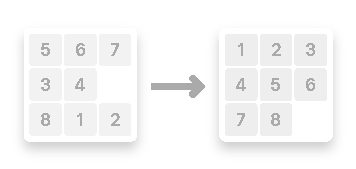
\includegraphics[keepaspectratio=true,width=10cm]{./inc/media/presentation_twoTaquins.pdf}
\caption{Un départ possible et l'arrivée voulue}
\label{presentationTwoTaquins}
\end{figure}

\paragraph{} {Les tuiles ne peuvent se déplacer que par glissement dans la seule case vide à un moment donné. Le jeu consiste à replacer les tuiles dans l’ordre numérique. Ainsi, par le biais de ce projet, nous allons donc, à l'aide du langage de programmation {\ttfamily Python}, développer ce jeu et répondre aux deux questions suivantes: Quelle est la séquence minimale de mouvements à faire sur un taquin pour obtenir la solution? Comment trouver cette séquence?}

\section{Etude du cas général}

\paragraph{}{Pour ce faire, nous détaillerons dans cette partie l’algorithme ${A*}$, prononcer A star, utilisé pour résoudre le problème, la définition des états et des actions que l’agent pourra réaliser dans chaque état puis nous aborderons spécifiquement la stratégie de recherche utilisée par l’algorithme dans le but d'obtenir une solution optimale.}

\subsection{Définition d’un état}

\paragraph{}{Afin de suivre précisément l’évolution de la résolution du problème, il convient de formaliser tout d’abord ce qu'est un état, et l'environnement dans lequel il évolue. Ainsi, par l'intermédiaire de la programmation orientée objet, nous pouvons définir l'environnement et les états par les attributs suivants:}

\paragraph{Environnement}
\begin{enumerate}
	\item [{\ttfamily\bfseries sizes}:] {les dimensions du taquin, largeur et taille}
	\item [{\ttfamily\bfseries choices}:] {les heuristiques choisies pour une exécution, soient les identifiants de chaque pondération ou de l'heuristique de la Mauvaise Place par exemple}
	\item [{\ttfamily\bfseries weightings}:] {les pondérations utilisées pour une exécution}
	\item [{\ttfamily\bfseries moves}:] {l'historique des coups joués par l'utilisateur}
	\item [{\ttfamily\bfseries end}:] {la solution trouvée par l'algorithme}
\end{enumerate}
\paragraph{Taquin}
\begin{enumerate}
	\item [{\ttfamily\bfseries environment}:] {l'environnement dans lequel évolue l’état}
	\item [{\ttfamily\bfseries previous}:] {la référence au taquin précédent – parent}
	\item [{\ttfamily\bfseries sequence}:] {l'ordre des tuiles dans le taquin, représenté par une liste, le vide vaut ${0}$; à l'état initial la {\ttfamily sequence} est une liste remplie aléatoirement}
	\item [{\ttfamily\bfseries inv}:] {le nombre d'inversions,  c’est-à-dire, le nombre de fois pour chaque élément de la {\ttfamily sequence}  où celui-ci est plus grand que chacun des éléments suivants}
	\item [{\ttfamily\bfseries dis}:] {l'abréviation de l'anglais {\em disorder}, désordre, soit le nombre de tuiles qui ne sont pas à la place occupée dans l'état final}
	\item [{\ttfamily\bfseries man}:] {la distance de Manhattan brute, n'ayant subie aucune pondération}
	\item [{\ttfamily\bfseries path}:] {le chemin emprunté par l'algorithme pour atteindre l'état actuel, réprésenté par une suite de lettres: {\ttfamily\bfseries L} pour gauche (left), {\ttfamily\bfseries R} pour droite (right), {\ttfamily\bfseries U} pour haut (up) et {\ttfamily\bfseries D} pour bas (down)}
	\item [{\ttfamily\bfseries moves}:] {la liste des prochains coups possibles à partir de l'état actuel}
	\item [{\ttfamily\bfseries h}:] {la somme des calculs de chaque heuristique utilisée}
	\item [{\ttfamily\bfseries g}:] {le côut d'un chemin allant de l'état initial à l'état actuel représenté par un entier}
	\item [{\ttfamily\bfseries f}:] {la fonction d'évaluation: ${f(n) = g(n) + h(n)}$ avec ${n}$ le taquin actuel}
\end{enumerate}

\subsection{Détail des heuristiques}

\paragraph{} {Dans le cadre de l'utilisation de l'algorithme ${A*}$, le choix d'heuristiques est nécessaire. De fait, nous aurons recours à 7 heuristiques, surestimant la longueur du chemin à parcourir pour atteindre l'état final. Les 6 premières sont des distances dérivées de la distance de Manhattan, correspondant aux heuristiques {\bfseries H.1}, {\bfseries H.2}, {\bfseries H.3}, {\bfseries H.4}, {\bfseries H.5}, {\bfseries H.6} et pondérées par les jeux de poids suivants:}
{\scriptsize\addfontfeatures{Numbers=Tabular}
\renewcommand{\arraystretch}{1.3}
\begin{center}
	\begin{tabular}
		{| c || c | c | c | c | c | c | c |} \hline & \textbf{1} & \textbf{2} & \textbf{3} & \textbf{4} & \textbf{5} & \textbf{6} & \textbf{7} & \textbf{8} \\

		\hline
	\end{tabular}
\end{center}}



\end{document}